%!TEX root = etdrtemplate.tex

\cleardoublepage


\chapter{PCA Pump}
\label{pcapump}

% http://www.santoslab.org/pub/paper/LarsonEtAl13-PCA-Requirements-SEHC-preprint.pdf
% http://ppahs.org/2012/05/30/patient-controlled-analgesia-pca-pumps-the-basics/

\begin{wrapfigure}{r}{0.4\textwidth}
  \begin{center}
    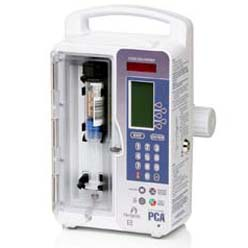
\includegraphics[width=0.4\textwidth]{figures/pca-pump.png}
  \end{center}
  \caption{Patient Controlled Analgesia (PCA) pump}
  \label{figure:pca-pump}
\end{wrapfigure}

Patient Controlled Analgesia (PCA) pump is a medical device, which allows the patient to self-administer small doses of narcotics (usually Morphine, Dilaudid, Demerol, or Fentanyl). PCA pumps are commonly used after surgery to provide a more effective method of pain control than periodic injections of narcotics. A continuous infusion (called a basal rate) permits the patient to receive a continuous infusion of pain medication. There is no need for a clinician to administer it. Patient can also request additional boluses, but only in specified intervals. It prevents from overinfusion. In addition to basal and patient bolus, clinician can also request bolus called clinician bolus or square bolus. 

Figure \ref{figure:pca-pump} shows LifeCare PCA pump. On the left hand side, there is drug reservoir. On the right -  clinician panel, which allows to control the pump. Figure \ref{figure:alaris-pump} shows PCA Pump, made by company Alaris. 

\begin{wrapfigure}{l}{0.4\textwidth}
  \begin{center}
    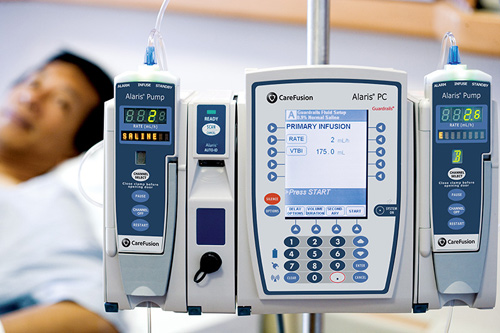
\includegraphics[width=0.4\textwidth]{figures/alaris-pump.png}
  \end{center}
  \caption{Alaris Pump}
  \label{figure:alaris-pump}
\end{wrapfigure}

PCA Pump is safety-critical device which works in standard process control loop depited in the figure \ref{figure:control-loop}. The controller obtains information about (observes) the process state from measured variables (feedback) and uses this information to initiate action by manipulating controlled variables to keep the process operating within predefined limits or set points (the goal) despite disturbances to the process. Such as different air pressure or device position (gravity impact). In general, the maintenance of any open-system hierarchy (either biological or man-made) will require a set of processes in which there is communication of information for regulation or control. \cite{SaferWorld} 

\begin{figure}[ht]%t=top, b=bottom, h=here
    \begin{center}
    	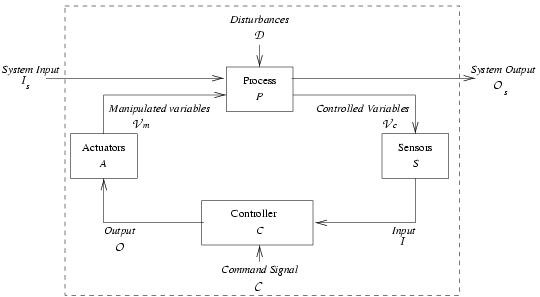
\includegraphics[width=0.9\textwidth]{figures/safety-critical-loop.png}    	
    \end{center}
    \caption{Standard Process Control Loop.}
    \label{figure:control-loop}
\end{figure}

PCA Pump actuator is motor, which pump drug to the patient's vein. Controlled process is dosing the drug. Sensors measure amount of dosed drug. They might be used for double-check if ordered (by controller) amount of drug was appropriately delivered. Sometimes there might be some distrubances caused by mechanical issues and environmental conditions. Controller issues appropriate actions based on informations from sensors and clinician or patient's commands. High level overview of PCA Pump is depicted in figure \ref{figure:pca-pump-system}.

\begin{figure}[ht]%t=top, b=bottom, h=here
    \begin{center}
    	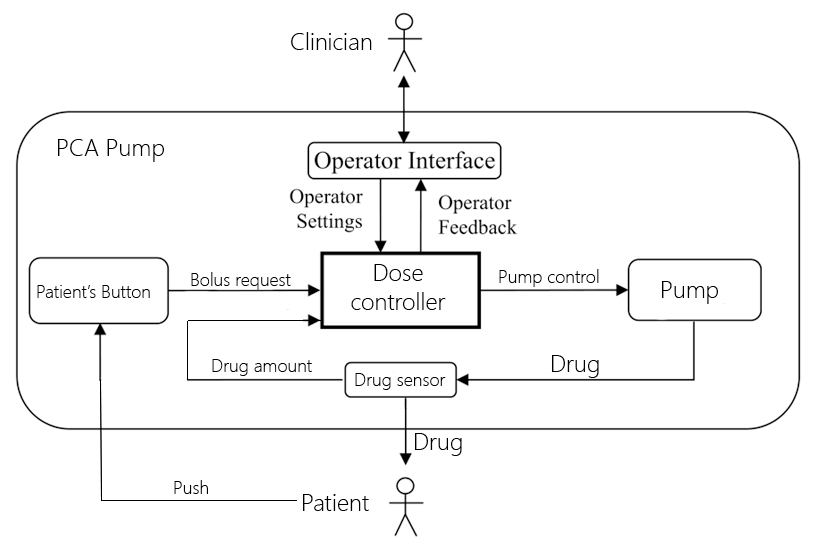
\includegraphics[width=0.9\textwidth]{figures/pca-pump-system.png}    	
    \end{center}
    \caption{PCA Pump system}
    \label{figure:pca-pump-system}
\end{figure}

One of the hazards of using PCA pumps, is that there is inadequate monitoring of patient's levels of oxygen and carbon dioxide. Nursing staff on general medical units typically track respiration rate and other vital signs every four hours, which is not enough. There should be a way to monitor levels continuously. Additionally, it can be hard to tell if a person's breathing rate is dangerously low in certain circumstances. There are cases, where lack of monitoring carbon dioxide level cause death.\footnote{http://abcnews.go.com/Health/parents-warn-pca-pumps-daughters-death/story?id=16796805} 

Another hazard is human mistake. For example, there is a case when nurse used a 5 mg/mL morphine cassette because a 1 mg/mL cassette was not available, but she programmed PCA Pump like for 1 mg/mL concentration. In addition to lack of monitoring of the pulse, patient died.\footnote{http://webmm.ahrq.gov/case.aspx?caseID=291}

As mentioned in chapter \ref{background}, the solution to that problem is medical devices interoperability. In addition, less human error-prone device is needed. 



\section{PCA Pump Requirements Document}
\label{pcapump:requirements-doc}

Requirements of Open PCA Pump are captured in "Integrated Clinical Environment Patient-Controlled Analgesia Infusion Pump System Requirements" document \cite{PcaReq} created by Brian Larson. It is formalized set of capabilities, which Open PCA Pump should have, based on consultations with domain experts, FDA and Brian Larson's expertise gained while he was working in the medical device industry.

Conceptual model of Open PCA Pump is depicted in the figure \ref{figure:ice-pca-pump}. As mentioned earlier, Pump is connected to ICE so it may be integrated with ICE apps and displays. The interface must provide prescription and patient information, current status to be displayed remotely on a supervisor user interface, and a means to stop infusing upon human command, or determination of an ICE app. Such an ICE app could monitor a patient's blood oxygenation and pulse rate, stopping the pump if depressed respiratory function is indicated. \cite{PcaReq}

\begin{figure}[ht]%t=top, b=bottom, h=here
    \begin{center}
      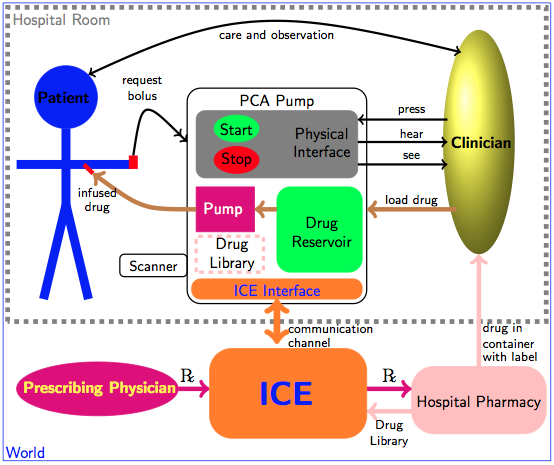
\includegraphics[width=0.9\textwidth]{figures/ice-pca-pump.png}      
    \end{center}
    \caption{Open PCA Pump concept}
    \label{figure:ice-pca-pump}
\end{figure}

Additionally, it cooperates with Drug Library, which contains information about drugs and its properties (like concentration). Data needed for pump operation, are captured on electronic prescription, which contains:
\begin{itemize}
    \item Patient's name
    \item Drug name
    \item Drug code
    \item Drug concentration
    \item Initial volume of drug in the vial
    \item Basal flow rate - the rate of continuous infusion
    \item Volume to be infused (VTBI) on patient's request
    \item Maximum amount of drug allowed per hour
    \item Minimum time between patient boluses
    \item Date, in which prescription has been filled
    \item Prescribing physician's name
    \item Pharmacist name
\end{itemize}

Pain medication is prescribed by a licensed physician, which is dispensed by the hospital's pharmacy. The drug is placed into a vial labeled with the name of the drug, its concentration, the prescription, and the intended patient. A clinician loads the drug into the pump, and attaches it to the patient. The pump infuses a prescribed basal flow rate which may be augmented by a patient-requested bolus or a clinician-requested bolus. This allows additional pain medication in response to patient need within safe limits. \cite{PcaReq}

Prescription captures all data needed for basal infusion and patient requested boluses (referred as bolus). In addition to that, Open PCA Pump allows Clinician Requested Bolus (refereed as square bolus). In order to do that, clinician has to enter the time (through PCA Pump panel) in which VTBI, specified in prescription, will be infused.

There can occur situations in which the maximum drug amount infused may exceed the allowed limit. E.g. when clinician issues too many square boluses. In such case, the Pump is switched to Keep Vein Open (KVO) mode, which has 1 ml/hr drug rate. Pump switches to KVO rate also when ICE interface request it. It may happen e.g. if patient's oxygen level is low. From KVO state pump has to be restarted by clinician in order to continue operation. In Summary, Open PCA Pump has following modes:
\begin{itemize}
    \item Stopped
    \item Basal rate
    \item Patient's bolus (bolus)
    \item Clinician bolus (square bolus)
    \item Keep Vein Open (KVO)
\end{itemize}

There are also other scenarios, which are captured by Requirements Document \cite{PcaReq}, like scanner to enable automatic entry of patient's and prescription data, occlusion detection, hardware errors etc. However, they are not part of this thesis and their overview is skipped.


[Add state machine image, like in UMinn Req Doc?]
% check UMinn document
[More details?]


More detailed overview of Open PCA Pump Requirements can be found in \cite{OpenSourcePCAPump:Paper}.


\section{PCA Pump AADL/BLESS Models}
\label{pcapump:aadl-bless-models}

In addition to PCA Pump Requirements Document \cite{PcaReq}, Brian Larson created AADL model with formal behavioral specifications written in his BLESS framework. AADL model, graphical representation is depicted on figure \ref{figure:pca-pump-aadl-model}. 

\begin{figure}%[h]%t=top, b=bottom, h=here
    \begin{center}
      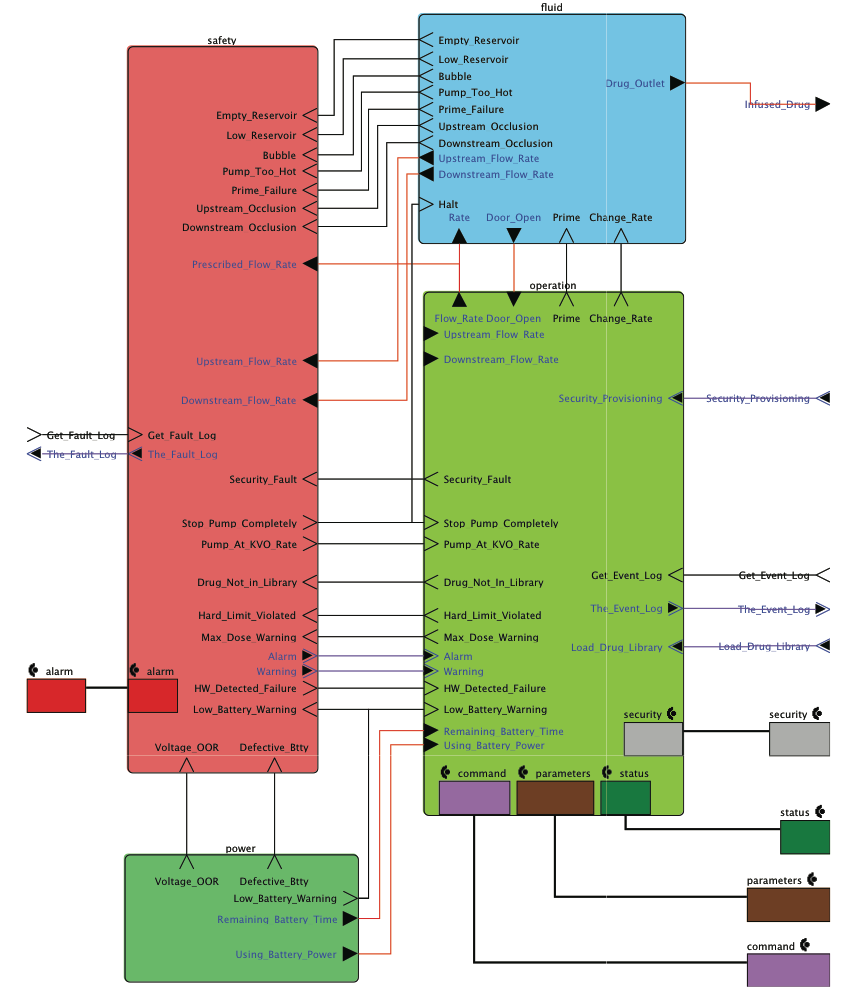
\includegraphics[width=0.9\textwidth]{figures/pca-pump-aadl-model.png}      
    \end{center}
    \caption{Open PCA Pump AADL model}
    \label{figure:pca-pump-aadl-model}
\end{figure}

AADL model captures structure of device. BLESS - its behavior. Listing \ref{listing:rate_controller} shows \lstinline{Rate_Controller} thread from \lstinline{PCA_Operation} component with BLESS assertions in thread declaration and BLESS behavioral description in thread implementation. The thread declaration contains input and output ports. In addition to some them, BLESS assertions are present. Assertions are defined in BLESS annex in thread implementation. In addition to assertions, states and transitions defined in thread implementation can potentially be translated into working SPARK Ada program. Presence of timing properties in states and transitions makes translation extremely difficult, thus there are omitted in this thesis and only assertions are considered.

\singlespacing
\begin{lstlisting}[language=aadl, frame=single, gobble=0, caption={\lstinline{Rate_Controller} thread from \lstinline{PCA_Operation} component with BLESS assertions}, label={listing:rate_controller}]
  thread Rate_Controller
  features
      Infusion_Flow_Rate: out data port PCA_Types::Flow_Rate
        {BLESS::Assertion => "<<:=PUMP_RATE()>>";};   
      System_Status: out event data port PCA_Types::Status_Type;
      Begin_Infusion: in event port
        {BLESS::Assertion => "<<Rx_APPROVED()>>";};  
      Begin_Priming: in event port;
      End_Priming: in event port;
      Halt_Infusion: in event port;
      Square_Bolus_Rate: in data port PCA_Types::Flow_Rate 
        {BLESS::Assertion => "<<:=SQUARE_BOLUS_RATE>>";};
      Patient_Bolus_Rate: in data port PCA_Types::Flow_Rate 
        {BLESS::Assertion => "<<:=PATIENT_BOLUS_RATE>>";};
      Basal_Rate: in data port PCA_Types::Flow_Rate 
        {BLESS::Assertion => "<<:=BASAL_RATE>>";};
      VTBI: in data port PCA_Types::Drug_Volume 
        {BLESS::Assertion => "<<:=VTBI>>";};
      HW_Detected_Failure: in event port;
      Stop_Pump_Completely: in event port; 
      Pump_At_KVO_Rate: in event port; 
      Alarm : in event data port PCA_Types::Alarm_Type;
      Warning : in event data port PCA_Types::Warning_Type;
      Patient_Request_Not_Too_Soon: in event port 
        {BLESS::Assertion => "<<:=PATIENT_REQUEST_NOT_TOO_SOON(now)>>";};  
      Door_Open: in data port Base_Types::Boolean;
      Pause_Infusion: in event port;
      Resume_Infusion: in event port;
      CP_Clinician_Request_Bolus: in event port;
      CP_Bolus_Duration: in event data port ICE_Types::Minute; 
      Near_Max_Drug_Per_Hour: in event port  --near maximum drug infused in any hour
        {BLESS::Assertion => "<<PATIENT_NEAR_MAX_DRUG_PER_HOUR()>>";};  
      Over_Max_Drug_Per_Hour: in event port  --over maximum drug infused in any hour
        {BLESS::Assertion => "<<PATIENT_OVER_MAX_DRUG_PER_HOUR()>>";};  
      ICE_Stop_Pump: in event port;
    properties
      Thread_Properties::Dispatch_Protocol => Aperiodic;
  end Rate_Controller;

  thread implementation Rate_Controller.imp
  annex BLESS
  {**
  assert
  --the infusion flow rate shall be:
  --  =0, after stop pump completely (from safety architecture), 
  --      clinician pressed stop button
  --  =KVO rate, after KVO rate command, or
  --      exceeded max drug per hour
  --      some alarms,
  --  =max rate, during patient-requested infusion
  --  =square bolus rate, during clinician-commanded infusion 
  --  =priming rate during pump priming
  --  =basal rate, otherwise
  <<HALT : :(la=SafetyPumpStop) or (la=StopButton) or (la=EndPriming)>>  --pump at 0 if stop button, or safety architecture says, or done priming
  <<KVO_RATE : :(la=KVOcommand) or (la=KVOalarm) or (la=TooMuchJuice)>>  --pump at KVO rate when commanded, some alarms, or excedded hourly limit
  <<PB_RATE : :la=PatientButton>>  --patient button pressed, and allowed
  <<CCB_RATE : :(la=StartSquareBolus) or (la=ResumeSquareBolus)>>  --clinician-commanded bolus start or resumption after patient bolus
  <<PRIME_RATE : :la=StartPriming>>  --priming pump
  <<BASAL_RATE : :(la=StartButton) or (la=ResumeBasal) or (la=SquareBolusDone)>>  --regular infusion
  <<PUMP_RATE : :=
    (HALT()) -> 0,                                      --no flow
    (KVO_RATE()) -> PCA_Properties::KVO_Rate,           --KVO rate
    (PB_RATE()) -> Patient_Bolus_Rate,  --maximum infusion upon patient request
    (CCB_RATE()) -> Square_Bolus_Rate,                  --square bolus rate=VTBI/duration, from data port
    (PRIME_RATE()) -> PCA_Properties::Prime_Rate,       --pump priming
    (BASAL_RATE()) -> Basal_Rate                        --basal rate, from data port
  >>
  invariant <<true>>
  variables
    --time of last action
    tla :BLESS_Types::Time := 0;
    la :   --last action
      enumeration ( 
        SafetyStopPump,   --safety architecture found a problem
        StopButton,       --clinician pressed stop button
        KVOcommand,       --from control panel (clinician) or ICE (app) to pump Keep-vein-open rate
        KVOalarm,         --some alarms should pump at KVO rate
        TooMuchJuice,     --exceeded max drug per hour, pump at KVO until prescription and patient are re-authenticated
        PatientButton,    --patient requested drug
        ResumeSquareBolus,--infusion of VTBI finished, resume clinician-commanded bolus
        ResumeBasal,      --infusion of VTBI finished, resume basal-rate
        StartSquareBolus, --begin clinician-commanded bolus
        SquareBolusDone,  --infusion of VTBI finished
        StartPriming,     --begin pump/line priming, pressed "prime" button
        EndPriming,       --end priming, pressed "prime" button again, or time-out 
        StartButton       --start pumping at basal rate
      );    
    pb_duration :BLESS_Types::Time  --patient button duration = VTBI/Patient_Bolus_Rate
      <<PB_DURATION : :pb_duration=(VTBI/Patient_Bolus_Rate)>>;
  states
    PowerOn : initial state;        --power-on
    WaitForRx : complete state;   --wait for valid prescription
    CheckPBR : state  --check Patient_Bolus_Rate is positive
      <<Rx_APPROVED()>>;
    RxApproved : complete state   --prescription verified
      <<Rx_APPROVED() and PB_DURATION()>>;
    Priming : complete state      --priming the pump, 1 ml in 6 sec
      <<(la=StartPriming) and (Infusion_Flow_Rate@now = PCA_Properties::Prime_Rate) and PB_DURATION()>>;
    WaitForStart : complete state   --wait for clinician to press 'start' button
      <<HALT() and (Infusion_Flow_Rate@now=0) and PB_DURATION()>>;
    PumpBasalRate : complete state  --pumping at basal rate
      <<((la=StartButton) or (la=ResumeBasal)) and (Infusion_Flow_Rate@now=Basal_Rate@now) and PB_DURATION()>>;
    PumpPatientButtonVTBI : complete state  --pumping patient-requested bolus
      <<(la=PatientButton) and PB_DURATION()
        and (Infusion_Flow_Rate@now=Patient_Bolus_Rate)>>;
    PumpCCBRate : complete state    --pumping at clinician-commanded bolus rate
      <<((la=StartSquareBolus) or (la=ResumeSquareBolus)) and (Infusion_Flow_Rate@now=Square_Bolus_Rate@now) and PB_DURATION()>>;
    PumpKVORate : complete state    --pumping at keep-vein-open rate
      <<((la=KVOcommand) or (la=KVOalarm) or (la=TooMuchJuice))  and PB_DURATION()
        and (Infusion_Flow_Rate@now=PCA_Properties::KVO_Rate)>>;
    PumpingSuspended : complete state  --clinician pressed 'stop' button
      <<((la=StopButton) or (la=SafetyStopPump)) and (Infusion_Flow_Rate@now=0)>>;
    Crash : final state;    --abnormal termination
    Done : final state    --normal termination
      <<Infusion_Flow_Rate@now=0>>;
  transitions
  --wait for valid prescription
    go : PowerOn-[ true ]->WaitForRx{};  
  --prescription validated
    rxo : WaitForRx-[ on dispatch Begin_Infusion ]-> CheckPBR{};
    pbr0 : CheckPBR-[ Patient_Bolus_Rate<=0 ]->Crash{}; --bad Patient_Bolus_Rate
    pbrok : CheckPBR-[ Patient_Bolus_Rate>0 ]->RxApproved
      {<<Rx_APPROVED() and (Patient_Bolus_Rate>0)>>  --likely will change from logic variable to predicate Rx_APPROVED()
        pb_duration := VTBI/Patient_Bolus_Rate  --calculate patient bolus duration
        --note division without knowing divsor is non-zero; should generate additional proof obligations for assignment using division
      <<Rx_APPROVED() and PB_DURATION()>>};  
  --clinician press 'prime' button
    rxpri : RxApproved-[ on dispatch Begin_Priming ]-> Priming  
      {
      la :=StartPriming
          <<Begin_Priming@now and Rx_APPROVED() and (la = StartPriming) and PB_DURATION()>>
      ; 
      Infusion_Flow_Rate!(PCA_Properties::Prime_Rate)  --infuse at prime rate
          <<(la = StartPriming) and Rx_APPROVED() and PB_DURATION() and
            (Infusion_Flow_Rate@now=PCA_Properties::Prime_Rate)>>   
      };
  --priming done, wait for start
    prd: Priming-[ on dispatch End_Priming or timeout (Begin_Priming) PCA_Properties::Prime_Time sec]-> WaitForStart  
      {
      la:=EndPriming
        <<HALT() and PB_DURATION()>>  --and Begin_Priming timed out
      ;
      Infusion_Flow_Rate!(0)   --stop priming flow
        <<HALT() and (Infusion_Flow_Rate@now=0) and PB_DURATION()>>
      };
  --prime again
    pri: WaitForStart-[ on dispatch Begin_Priming ]-> Priming  
      {
      la:=StartPriming
          <<Begin_Priming@now and PB_DURATION() and PRIME_RATE()>>
      ; 
      Infusion_Flow_Rate!(PCA_Properties::Prime_Rate)  --infuse at prime rate
          <<PRIME_RATE() and PB_DURATION() and
            (Infusion_Flow_Rate@now=PCA_Properties::Prime_Rate)>>   
     };
  --clinician press 'start' button after priming    
    sap: WaitForStart-[ on dispatch Begin_Infusion ]-> PumpBasalRate  --start after priming
      {
      la:=StartButton
        <<(la=StartButton) and Begin_Infusion@now  and PB_DURATION()>>    
      ;
      Infusion_Flow_Rate!(Basal_Rate)   --infuse at basal rate
        <<(la=StartButton) and (Infusion_Flow_Rate@now=Basal_Rate@now) and PB_DURATION()>>
      };
  --Patient_Request_Bolus during basal rate infusion
    pump_basal_rate: 
    PumpBasalRate-[ on dispatch Patient_Request_Not_Too_Soon]-> PumpPatientButtonVTBI
      {
      la := PatientButton 
        <<(la=PatientButton) and Patient_Request_Bolus@now and PB_DURATION()>>    
      ;
      Infusion_Flow_Rate!(Patient_Bolus_Rate)   --infuse at patient button rate
        <<(la=PatientButton) and PB_DURATION()
          and (Infusion_Flow_Rate@now=Patient_Bolus_Rate)>>     
      };  --end of pump_basal_rate
  --VTBI delivered
    vtbi_delivered: 
    PumpPatientButtonVTBI -[ on dispatch timeout (Infusion_Flow_Rate) pb_duration ms ]-> PumpBasalRate
      {
      la:=ResumeBasal
      ;
      <<(la=ResumeBasal) and PB_DURATION()>>  --and timeout of patient button duration
      Infusion_Flow_Rate!(Basal_Rate)   --infuse at basal rate
        <<(la=ResumeBasal) and (Infusion_Flow_Rate@now=Basal_Rate@now) and PB_DURATION()>>   
      };  --end of vtbi_delivered
  **};
  end Rate_Controller.imp;
\end{lstlisting} 
\doublespacing

\section{BeagleBoard-XM}
\label{pcapump:beagleboard}

\begin{wrapfigure}{r}{0.5\textwidth}
  \begin{center}
    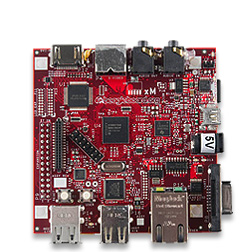
\includegraphics[width=0.5\textwidth]{figures/beagleboard_xm.png}
  \end{center}
  \caption{BeagleBoard-xM}
  \label{figure:beagleboard_xm}
\end{wrapfigure}

For Research and MDCF purposes, BeagleBoard-xM (an open-source hardware single-board computer produced by Texas Instruments), has been chosen as hardware platform for PCA Pump prototype.

BeagleBoard-xM is Embedded device with AM37x 1GHz ARM processor (Cortex-A8 compatible). It has 512 MB RAM, 4 USB 2.0 ports, HDMI port, 28 General-purpose input/output (GPIO) ports and Linux Operating System (on microSD card). Moreover there is PWM support, which enables control of pump actuator. All these properties makes this device good candidate for prototyping PCA Pump.

Pulse-width modulation (PWM) is a technique for controlling analog circuits with a processor's digital outputs. The average value of voltage (and current) fed to the electrical load is controlled by turning the switch between supply and load on and off at a fast pace. The longer the switch is on compared to the off periods, the higher the power supplied to the load. Proportion of on and off periods is called the duty cycle and is expressed in percent. 100\% means all the time on, 0\% - all the time off. Figure \ref{figure:pwm} shows 10\%, 30\%, 50\% and 90\% duty cycles.

\begin{figure}[ht]%t=top, b=bottom, h=here
    \begin{center}
      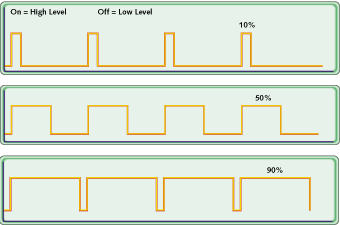
\includegraphics[width=0.9\textwidth]{figures/pwm.png}      
    \end{center}
    \caption{An example of PWM duty cycles}
    \label{figure:pwm}
\end{figure}

There is no existing SPARK Ada compiler running on ARM system. Hence, to compile SPARK Ada program for ARM device, cross-compiler is needed. There is GNAT compiler \cite{Horn:Thesis} created by AdaCore, but there was no cross-compiler for ARM. However, AdaCore was actively developing cross-compiler. They had working version in 2013, but tested only on their target Android-based device. In cooperation with AdaCore, cross-compiler for ARM was bundled and tested on BeagleBoard-xM. For now, GNAT cross-compiler works only on Linux 32-bit operating system.

In addition to USB ports, BeagleBoard-xM has also serial port and Ethernet port. It allows to copy programs compiled on Linux, using all three, mentioned types of ports. 
